\documentclass{tufte-handout}
\usepackage{graphicx}
\usepackage{listings}
\graphicspath{ {./img/} }
\author{Andr\'es Ponce}
\title{Main Memory}

\begin{document}

\begin{abstract}
Here we look at how our operating system can place the currently executing programs
at least partially in memory, and how the memory management contributes to 
normal execution.
\end{abstract}

When we execute a program, the data to be used by that program has to first be in the
registers coupled with the CPU. During the instruction exection cycle, the CPU
will fetch the data from these addresses. If the instruction requires data from 
memory, then that data has to be brought over to the CPU before it's used.

The problem comes when we have to wait for the information to arrive at 
the CPU registers. Instead of having to go all the way to main memory every time 
we want to access some memory, we can also have some levels of memory closer to the 
CPU. Instead of having to go all the way to main memory every time 
we want to access some memory, we can also have some levels of memory closer to the 
CPU. This \textbf{cache} can then speed up subsequent memory accesses.

In actual memory, our processes have to have their own address space. This is done 
to ensure that processes can't access each other's memory space and so that 
each process only has a set size. There are two registers, the \textbf{base} and
\textbf{limit} registers, which store the beginning and end of the address space for 
each process. 

When we CPU generates an address, it has to be checked with the base and limit 
registers to make sure that the address is valid.

When we CPU generates an address, it has to be checked with the base and limit 
registers to make sure that the address is valid. If the program tries to modify 
invalid addresses, then it will be sent as a trap to the operating system and 
the program will be removed from memory.

\section{Address binding}

When a program gets loaded into memory, it need not be in numerical order, it could 
be loaded at any available location. Thus there has to exist a process by which
we can map some addresses from a logical perspective to the hardware. In the source
program, such addresses are usually symbolic, meaning that during the compilation process
usually we don't use the physical addresses. Once the linker is activated, it will 
map the addresses used by the loader and compiler and replace them with the actual 
physical addresses. However, this binding can be done at any step in the compilation
process. 

\begin{itemize}
	\item \textbf{Compile Time}: If we know which address the program will start in, 
			then we can just calculate all the addresses manually. However, we usually
			don't know where the program will be loaded.
	\item \textbf{Load Time}: If we don't know where the program will be loaded, then 
			we have to "fill in the blanks" when the program is loaded. For example, 
			we could just calculate all addresses based on the initial address, and 
			when we load the program and thus know the initial address, we can update
			the remainder of the addresses.
	\item \textbf{Run Time}: We could wait until the program is running to assign addresses
			if the program segment could be moved during execution. However, we would
			need special hardware to do this but apparently that's how it's done 
			in modern operating systems.
\end{itemize}

The addresses used by the CPU are called \textbf{virtual} (logical) addresses. The 
\textbf{Memory Management Unit(MMU)} is the entity responsible for actually carrying 
out the conversion. The base register, which holds the initial possible address, is called the \textbf{relocation register}. This register's value is then added to all the addresses sent to the memory. So the CPU would deal with "offsets" and the 
relocation register is the amount they're offset to. So if the initial address
is 14,000, and we want to access memory value 436, we would map it to the physical 
address 14,436.

This has the effect that the user  program never really deals with physical addresses. 
Even when we use pointers and "interact with memory" all those instructions still have
to pass through the MMU.
\footnote{Maybe by differentiating logical/physical addresses, we also remove the 
limitation of how big our memory address can be, since the MMU would know what the 
maximum address is.}

\textbf{Dynamic Loading} refers to loading some parts of our code when they're needed
rather than loading it all at the same time. When our program wants to execute 
a certain routine, we have to check if the routine has been loaded or not. If it hasn't,
we have to fetch it from memory and update the address tables to reflect the change.

\textbf{Dynamically Linked Libraries} are files that are linked to the user program
when they are called. This is typically done for system libraries such as those in C.
Instead of including the entire library, we can only call the required routines. In 
Linux these are \textbf{shared libraries}. We can also used shared libraries
to update versions of the library. If we just have a new version of the library, 
the program will automatically use the new version of the library. However, to 
prevent a user program from using an incompatible version of the library, we can 
embed version information within the library so that the user program and operating
system avoid using this version.

\section{Coniguous Memory Allocation}
This memory allocation scheme involves placing processes in contiguous areas of 
memory. The operating system can also be placed in different positions in 
memory. It can be placed in low addresses or high addresses.
\footnote{This also depends on the interrupt vector}Most operating systems now 
place the code in the higher addresses.

\begin{marginfigure}
	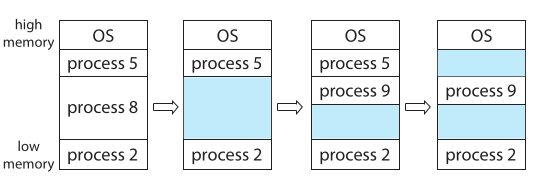
\includegraphics{partition}
	\caption{In a \textbf{variable partition scheme}, we can have multiple
			processes that are in different sections of memory, provided we 
			load the appropriate relocation and limit register.}
\end{marginfigure}

In a variable allocation scheme, we have \textbf{memory holes}, which refers to the 
space between two occupied regions of memory. When a process comes in ready to be 
scheduled, we choose a hole to load the program in. The hole is thus split in two,
the part of the hole occupied by our program, and the area of the hole that remains 
free. This second part is returned to the set of free holes.

There are a couple of ways of deciding how to assign processes to available memory 
space:
\begin{itemize}
	\item \textbf{First Fit}: Assign the process to the first hole that can fit 
				it. We can start searchign sequentially from the beginning every time
				or from the location where it last stopped.
	\item \textbf{Best Fit}: Assign the process to the smallest hole that fits it. 
				If the holes are not ordered by size, we would have to search the 
				entire space.
	\item \textbf{Worst Fit}: Assign the largest hole to each program. Might have to 
				search the entire space again, however might leave more contiguous
				space for some other programs.
\end{itemize}
Using the best fit or first fit approach suffers from \textbf{external fragmentation}.
This means that as processes get loaded and removed from memory, there will be smaller
and smaller pieces of contiguous memory that are unused. For example, suppose we want
to add a new process, we might have a situation where there is enough free memory in
total to add a process, but it is not conitguous, so the process cannot all fit in 
one place.

A possible solution to this might be to split memory into smaller partitions called
\textbf{blocks}. Blocks might then be given to programs and the leftover memory within
a block might in the end be less than if we jsut assigned contiguous memory without
partiitoning it. \textbf{Internal Fragmentation} is the difference between the size
of a memory block and the size of a process on that block. 

A technique which can sometimes help with external fragmentation is \textbf{compaction}.
Using this scheme, we could try and move all the free blocks of memory together into
one large hole, having a "tight fit" of the process memory space. However, this can 
only be done if the addresses are figured out dynamically during execution, since 
we might need to relocate the entire program around. Remember that if we can change 
the base register during execution and then update all the addresses automatically,
then we can pull this off.

Another solution, and the one that is used most frequently, is called \textbf{paging}.
Paging removes the limiation of a process to all reside in continuous memory, and 
so allows us to split a process and locate it wherever there is space available.

Logical memory is broken down into \textbf{pages} and physical memory is broken down into
\textbf{frames}. This means that the physical address in memory is completely separated
from logical memory. When a process is loaded into memory, we move the generate two values:
the \textbf{page number} and the \textbf{page offset}. Then, the memeory unit keeps a 
page table where we can convert from logical addresses to physical frame number.
One part of the logical addresses used by the CPU might refer to the offset from the page
number.

\begin{marginfigure}
	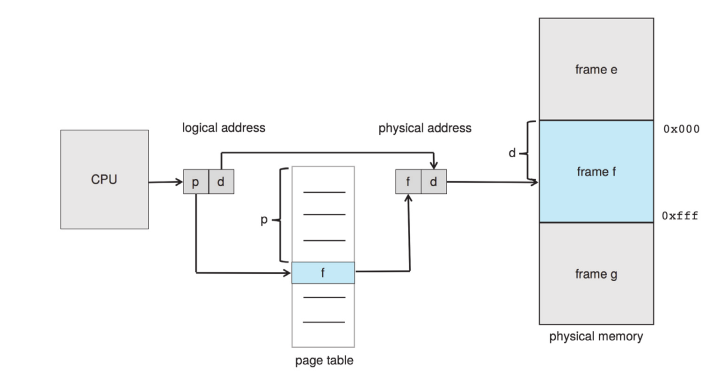
\includegraphics[scale=0.2]{paging.png}
	\caption{Part of the logical address will be composed of the page number $d$ and the offset
		within that page $d$. Once the MMU converts $d$ to the corresponding physical frame $f$
		in main memory, we can get the address by adding $f + d$.}
\end{marginfigure}

The system keeps its own data structure where we store the information about pages on our 
system is called \textbf{page table}. There is also one copy of the page table kept for
each of the processes that are run, so paging increases context switch time. However, 
we can directly change the \textbf{page-table base register}, which directly points to the 
table, to save time in querying/changing the table. However, when we access this table 
for each memory access, we have to in essence perform two memory accesses, which doubles
the number of accesses in total.

A solution to this is to have a small buffer, called the \textbf{transition look-aside buffer}.
This buffer is an associative space where we can check the corresponding field for some key.
We can check all the values in this buffer simultaneously, so we are essentially not adding
any performance.

Every entry in the page table has a bit known as \textbf{valid-invalid} bit. This means that
this entry is in the process's valid address range.\footnote{So is there one comparing 
every process to every other process?}

For every piece of system code, we might need to include code that never changes. For example
\texttt{libc} never changes during execution and many processes need it, so we might let 
all the processes use the actual library instead of having to copy all the code each time 
a process uses it. 

\section{Structure of The Page Table}
Given that the logical address space of a program might be 32 bits, this would mean that the 
logical page space might be too big if we have many processes. An alternative to this would 
be to \textit{page the page table}. Thus, if we previously had 20 bits of the logical address
indicate the page number and 12 for the offset, we could have the first 10 and second 10 bits
indicate the page number and the page within the page, respectively. The second part still 
remains the offset.

We can also use a hash table to map the virtual addresses to the page table.

\section{Swapping}

This refers to passing one process from main memory to secondary storage.
Modern OSs usually swap a page, rather than an entire process, since the 
latter might be too big to make it feasible.
\end{document}
